\documentclass[]{article}

\usepackage[margin=1in]{geometry}
\usepackage{amsmath}  % needed for \tfrac, \bmatrix, etc.
\usepackage{amsfonts} % needed for bold Greek, Fraktur, and blackboard bold
\usepackage{graphicx} % needed for figures
\usepackage{setspace}
\usepackage{times}
\usepackage{relsize}
\usepackage{framed}
\usepackage{float}
\usepackage{subfig}
\usepackage{color}
\usepackage{subcaption}

\begin{document}
	\title{XCP Computational Physics Workshop Final Report Draft}
	\author{Scott Campbell}
	\date{\today}

	\maketitle

\section{Chapter Abstract}
  The Thermal Radiative Transfer (TRT) equations describe the coupling between thermal radiation and material, which is an important physical process in many problems of interest to the astrophysics community. The Implicit Monte Carlo (IMC) method, originally developed over 40 years ago \cite{FC71}, is a standard solution methodology for the TRT equations.
  In this research, an improvement for IMC techniques for analyzing the interactions between a supernova and its circumstellar material is discussed, tested, and analyzed for a simplified geometry. This improvement uses a response function based variance reduction method to better estimate the observed time-dependent signal from a supernova system. The response function method improves the convergence, reliability, and accuracy of the IMC simulations. We were able to demonstrate said improvements by implementing this method in the open-source branson IMC code developed by Alex Long (\textit{along@lanl.gov}) using modern object-oriented languages.

\section{Introduction}
  Some ideas to add here:
  \begin{itemize}
    \item What is the supernova problem? Why is it difficult to obtain good tallies for supernova problems using IMC?
    \item Why is it important to improve efficiency for supernova simulations? (e.g. problem scale is large in space and time, so very computationally expensive... multiple physics involved that need to be modeled, etc.)
    \item (Very briefly) What are some of the basic variance reduction methods that people have used to try to improve efficiency for Monte Carlo? Mention weight windows / modified sampling -- then mention that you will describe them in more detail later
  \end{itemize}

  \textcolor{red}{RYAN: Here are two paragraphs for the first two points above (feel free to modify).}
  Electromagnetic (EM) transients are the main observational probe of supernovae, providing insight into the explosion energy, dynamics, and
  compositions of the exploding stars.
  These transients are formed by the complex interaction of photons with matter expanding at high velocity, and with a circumstellar medium
  (CSM) that existed before the supernova.
  Modeling supernovae with CSM interactions in multiple dimensions and extracting numerical transients is a challenging computational problem,
  requiring high spatial resolution in areas, relative to the overall distance between the star and CSM~\cite{MS10,MB13}.
  For the radiative transfer, in 1D deterministic~\cite{MB13} and Monte Carlo~\cite{KW09} have been applied to synthesize light curves and
  spectra.
  However, to our knowledge, for 2D and 3D only simplified treatments of the radiation have been employed: parameterized radiative
  cooling~\cite{MS10,MK12}, the M1 moment closure approximation~\cite{VL16}, or no treatment (only hydrodynamics)~\cite{MP18}.
  Nevertheless, apherical (or multidimensional) geometry can significantly impact the properties of the EM transient (spectra, light curves)
  \cite{VL16,MP18}, and the effect of higher-order radiative transfer on the observables may be non-negligible.

  Monte Carlo lends itself well to multiple dimensions, since the sourcing of particles in space can adjusted to mitigate transport in low-energy
  regions.
  In a simulation of a multidimensional supernova interacting with a CSM, obtaining well-sampled multi-frequency, multi-observer-angle
  spectra may generally be prohibitively expensive with Monte Carlo, assuming escaping particles are directly tallied as part of the transient.
  For instance, assuming a modest $100^3$ cell 3D simulation, 10 observational views, and 100 observational wavelegnth bands, and further assuming
  1\% of particles from each cell are tallied as escaping flux, the potential number of particles required to obtain 1 tally in each point in the
  observational phase space would be $\sim 100^3 \times 10 \times 100 \times 100 = 10^{11}$ particles.
  Given the expense of simulating this number of particles, variance reduction that takes into account statistics at a tally surface
  (i.e. the ``telescope'') is worth exploring.

	The remainder of this report outlines the background, motivation and theory for the method, the algorithmic procedure, initial results, and an analysis of the cases and conditions where the method is useful.


\section{Background and Theory}
	\subsection{Thermal Radiation Transport}
		The scattering and absorption of photons emitted from a material is described by the TRT equations:
		\begin{equation} \label{Eq: TRT_1}
		\frac{1}{c} \frac{\partial I}{\partial t}(\vec{r}, \vec{\Omega}, \nu, t) + \vec{\Omega} \frac{\partial I}{\partial \vec{r}}(\vec{r}, \vec{\Omega}, \nu, t) + \sigma_{a}(\vec{r}, \nu, T)I(\vec{r}, \vec{\Omega}, \nu, t) = 2 \pi \sigma_{a}(\vec{r}, \nu, T)B(\nu, T) + \frac{Q}{2}(\vec{r}, \nu, t),
		\end{equation}
		\begin{equation} \label{Eq: TRT_2}
		c_{v}(\vec{r}, T) \frac{\partial T}{\partial t}(\vec{r},t) = \int_{0}^{\infty} \int_{-1}^{1} \sigma_{a}(\vec{r}, \nu^{\prime}, T)[I(\vec{r}, \vec{\Omega}^{\prime}, \nu^{\prime}, t) - 2 \pi B(\nu^{\prime}, T)] d \vec{\Omega}^{\prime} d \nu^{\prime}
		\end{equation}
		where $I$ is the specific intensity, $T$ is the material temperature (keV), $c$ is the speed of light, $B$ is the Planck function, $Q$ is the inhomogenous source, $c_{v}$ is the material specific heat, and $\sigma_{a}$ is the absorption opacity. Each of the terms in Eq. \ref{Eq: TRT_1} corresponds to a loss or gain of photons from some phase space of the radiation field. The first term describes how the time behavior of the specific intensity depends on different gains and losses. The second is the streaming term, which describes how photons are lost by spatial streaming out of the phase space. The third describes the loss due to absorption into the material. On the right-hand side, the first is a gain term describing the radiation source from material temperature, and the second term then describes an arbitrary source of radiation. Equations \ref{Eq: TRT_1} and \ref{Eq: TRT_2} are non-linearly coupled by the material temperature.

	\subsection{Implicit Monte Carlo}
		Monte Carlo methods are used to model time-dependent, nonlinear, radiative transfer problems in complex three-dimensional configurations. This stochastic numerical method uses random sampling to determine where and how a particle moves through a material. Some Monte Carlo methods minimize the effects of discretization errors through a continuous treatment of energy, space, and/or angle leaving the primary errors to be rooted in stochastic uncertainties. However, Monte Carlo methods typically come at the expense of long run times (with a standard convergence rate $\propto\frac{1}{\sqrt{N}}$, where $N$ is the number of histories simulated) and heavy use of machine resources.

		The Implicit Monte Carlo (IMC) method is a specific variant of Monte Carlo originally developed by Fleck and Cummings in 1971 to solve the TRT equations \cite{FC71}. IMC uses `effective scattering' to model particle absorption/re-emission in a material for its current time step. This is represented by the Fleck factor, $f$, described as follows:
		\begin{equation}
			f = \frac{1}{1 + \frac{4acT^{3}\sigma \Delta t}{c_{v}}}
		\end{equation}
		where $a$ is the radiation constant, $c$ is the speed of light, $T$ is the material temperature, $\sigma$ is the material opacity, $\Delta t$ is the time step, and $c_{v}$ is the material specific heat.

		The IMC method applies two note-worthy approximations: semi-implicit discretization of time, and the linearization of the TRT equations. By linearizing the TRT equations, IMC is known to lead to inaccurate or non-physical results. Additionally, the time discretization is not fully implicit as implied, but rather semi-implicit as it is typically too expensive to converge otherwise.

    In the \textit{branson} IMC code used for this research, the spatial domain is discretized into rectangular regions referred to as cells, each with a constant material temperature, radiation temperature, and density per timestep. Particles are tracked as they move through the cells and can be absorbed into the material, scattered, or stream out of the spatial domain. A particle is transported until it reaches the end of the time step or is fully absorbed by the material. Information about the system (e.g. fluence) is accumulated during the timestep and stored in a `tally'.


	\subsection{Variance Reduction for IMC}
		Since the IMC method is stochastic, there will always be some statistical error in the result. Inherent issues with IMC methods include slow convergence and large computational requirements [CITE]. Furthermore, in cases where a material is optically thick and the distance from source to observation point (i.e. a tally surface) is large enough, the analog IMC method will fully absorb most particles into the material before they reach the tally, leaving the tally poorly sampled.

		Due to these issues, variance reduction methods for IMC methods are necessary to provide equivalent answers while using less resources and converging faster. In the IMC code used, three standard variance reduction techniques were incorporated in addition to the response function method. Currently, there are a large variety of variance reduction methods suited to different purposes. Common examples include implicit capture coupled with history termination, splitting and russian roulette, exponential transformation, forced collisions, source biasing, correlated sampling, optical reciprocity, and weight windows [CITE].

		Implicit capture is a standard method implemented in the \textit{branson} code. Implicit capture, or absorption supression, adjusts particles weight at every `scattering' event according to the following relationship:
		\begin{equation}
			w_{n,~i+1} = w_{n,~i}(1 - \frac{\sigma_{a}}{\sigma_{a} + \sigma_{s}})
		\end{equation}
		where $\sigma_{a}$ and $\sigma_{s}$ are the absorption and scattering cross-sections respectively. Using the Fleck factor, the above becomes
		\begin{equation}
			E_{particle,~i+1} = E_{particle,~i}e^{-\sigma_{a} \cdot f \cdot d_{event}},
		\end{equation}
		where $d_{event}$ is the distance to the next position the particle travels to. Implicit capture allows particles to stay active longer, increasing the likelyhood that a particle reaches the tally surface.

		Weight windows are another common variance reduction technique, in which each cell in the problem mesh is given a weight window center bounded by higher and lower values [CITE]. Once a particle enters a new cell, if a particles weight is not within the weight window, one of two processes will occur. If the particle's wright is above the window, it will be split into additional particles. Particles whose weight is below the window will undergo a technique such as Russian Roulette [CITE] to remove the particle from the simulation.

		All of the variance reduction methods listed above do not ensure that a tally surface will always be well sampled. In cases where particles have short mean free paths (i.e. traveling through a material with a high opacity), particles are still not guaranteed to pass through the tally surface. To ensure a tally is  well-sampled, ideally all particles would contribute to the tally at least once before being fully absorbed into the material. To this end, a response function in theory will meet this requirement.

	\subsection{Next Event Estimators}
		Next event surface crossing estimators (NXTEVT) are a standard method for analyzing Monte Carlo methods. NXTEVT contributes to a tally surface the expected value of a partilce that will cross through the tally surface. This method is an effective tool to minimize variance in situations where particles have limited histories, and large mean free paths in the problem material [CITE].

		Assuming that a particle is at a position $\vec{r}$, direction $\vec{\Omega}$, and weight $w_{0}$ intersecting a tally with a surface area $S_{tally}$ at a position $\vec{r^{\prime}}$ from the particle, the scored flux $\phi(\mu)$ is given by
		\begin{equation}
			\phi(\mu) = w_{0} \frac{e^{-\int_{\vec{r}}^{\vec{r^{\prime}}} \Sigma_{t}(s)ds}}{S \cdot \mu}
		\end{equation}
		where $\mu$ is the angle between $\vec{\Omega}$ and the surface normal at $\vec{r^{\prime}}$, and $\Sigma_{t}$ is the total cross section in the material.

	\subsection{Response Function Theory}
		A response function is thought to be an effective variance reduction method since it contributes an adjusted energy value to the tally at every scatter event, rather than adding a contribution only once the particle passes through the tally surface. Because of this feature, the tally surface should be well sampled using the response function compared to standard variance redution methods.

		A response function attempts to calculate the probability that a particle `survives' to the tally surface following its current trajectory. The weight of the particle based on this probability and current energy should the particle reach the tally surface is calculated by

		The response function is generated by tracing a number of particles through the problem domain starting uniformly on the tally surface, directed at a cosine-distribution angle. Since each cell may have a unique $\sigma_{a}$, every possible path from the source to the tally surface will result in a potentially unique contribution to the tally. The response function attempts to model this by averaging the absorption opacity based on the accumulation of all weighted $\sigma_{a}$ values from the previous cells into an effective opacity, $\sigma_{r}$. At every scattering event, the particles contribution to the tally is calculated by

		\begin{equation}\label{Eq: tally_contr}
		E_{contribution} = E_{particle}e^{-(\sigma_{r} + \frac{1}{c \Delta t})d_{tally}}
		\end{equation}
		where $E_{particle}$ is the current energy of the particle, $\Delta t$ is the current time step, and $d_{tally}$ is the distance of the particle to the tally surface along its path.

	\subsection{Supernova and CSM Parameters} \label{sec:sncsmpars}
		We attempt to model a snapshot of a supernova interacting with a circumstellar medium (CSM). The CSM has high enough mass to theoretically produce a superluminous supernova (e.g. SN 2006gy). The time for the snapshot is chosen to be after the supernova ejecta hits the CSM and produces a shock. This shock ionizes the CSM, which increases the opacity and consequently the optical depth. Moreover, the increase in density from the shock, coincident with the ionized region, also contributes to an increase in the optical depth of the CSM.

		The approximate properties of each layer near the time of peak luminosity ($\sim70$ days) for model D2 of Moriya, Blinnikov, et al (2013) (hereafter M13) are as follows.

		Supernova ejecta:
		\begin{itemize}
			\item $R_{\rm s, min} = 0$ cm
			\item $R_{\rm s, max} = 10^{15.829}$ cm
			\item $\rho_{\rm ej} = 10^{-14}$ g/cm$^3$
			\item $T_{\rm ej} = 10^4$ K
			\item $c_v = 10^6$ erg/K/g
			\item $\kappa_{\rm ej} = 0.3$ cm$^2$/g
		\end{itemize}

		Ejecta-CSM shock:
		\begin{itemize}
			\item $R_{\rm s, min} = 10^{15.829}$ cm
			\item $R_{\rm s, max} = 10^{15.831}$ cm
			\item $\rho_{\rm s} = 10^{-12}$ g/cm$^3$
			\item $T_{\rm s} = 10^6$ K
			\item $c_v = 10^6$ erg/K/g
			\item $\kappa_{\rm s} = 0.3$ cm$^2$/g
		\end{itemize}

		CSM (pre-shock):
		\begin{itemize}
			\item $R_{\rm s, min} = 10^{15.831}$ cm
			\item $R_{\rm s, max} = 10^{16}$ cm
			\item $\rho_{\rm CSM} = 10^{-14}$ g/cm$^3$
			\item $T_{\rm s} = 10^4$ K
			\item $c_v = 10^6$ erg/K/g
			\item $\kappa_{\rm CSM} = 10^{-4}$ cm$^2$/g
		\end{itemize}

		For spherical symmetry, these values give masses of about 6, 8.5, and 14 for the interior ejecta, shocked ejecta-CSM, and CSM, respectively, which are on the order of the model values presented by M13. The optical depth through the internal ejecta is about 20, and is about 10 through the shocked ejecta-CSM layer. The preshock CSM is evidently hot enough to be ionized, hence it can contribute another 10 mean-free-paths of optical depth. The spatial width of the shock layer is only 0.46 \% of the radius of the shock, despite providing 1/3 of the total optical depth.

	\subsection{Rescaling Parameters} \label{sec:rescaling}
		We may scale adjust dimensions and scale the parameters to simplify setup of input. This can also be of use when attempting to test different types of supernovae conditions, but preserving physical properties or numerical resolution.

		An adjustment of the overall domain size (radius),
		\begin{equation}
			\frac{R}{R_0} \approx 10^{-16} \;\;,
		\end{equation}
		where values subscripted with $0$ are unscaled, gives dimensions of O(1 cm). Relevant properties to preserve are the optical depth, light crossing time, and ratio of total time to the absorption-emission timescale. To preserve the light crossing time, we simply scale the total simulation time,
		\begin{equation}
			t = \frac{R}{R_0}t_0 \;\;,
		\end{equation}
		Similarly, assuming opacity is constant or piecewise-constant, the optical depth is preserved when
		\begin{equation}
			\kappa = \kappa_0\frac{R_0}{R} \;\;,
		\end{equation}
		where density has canceled from the left and right side. To preserve the ratio of the absorption-emission time scale to the total time, $t$,
		\begin{equation}
			t_{ae} = \frac{c_v}{4\kappa acT^4} = \frac{R}{R_0}t_{ae,0}
			= \frac{R}{R_0}\frac{c_{v,0}}{4\kappa_0 acT^4} \;\;,
		\end{equation}
		which implies
		\begin{equation}
			c_v = c_{v,0} \;\;.
		\end{equation}

		Density and temperature have been left unchanged. The important aspect of this problem is the geometric structure and optical depth. To lower the spatial resolution requirements, the ejecta-CSM shock layer may be spread from 0.4\% to $\sim$10\% of the problem length while preserving optical depth. To do so, the density of the layer can be lowered to compensate for the increased size of the layer.

\section{Method and Technical Approach}
	\begin{figure} [h!]
		\centering
		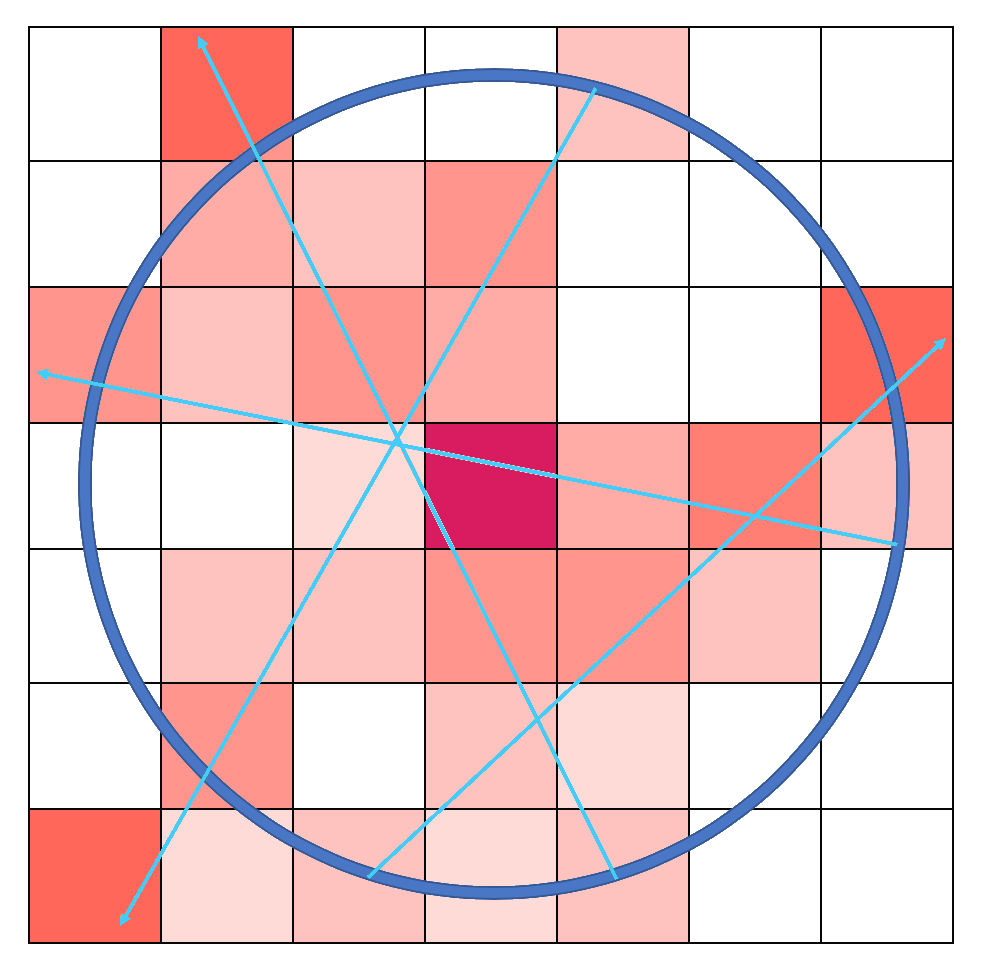
\includegraphics[height=3in]{Figures/resp_funct_pt_src_vis.png}
		\caption{A simplified visualization of the response function method. Particles are traced from the surface of the tally (blue ring) ‘towards’ the source (purple square) until they exit the mesh. As the particle moves, an adjusted opacity, $\sigma_{r}$, is calculated based on how far the particle has traveled from its origin on the tally surface, as well as the $\sigma_{a,~cell}$ values of the cells that it has passed through. A darker shade of red corresponds to a higher $\sigma_{r}$ value – a less likely chance that a particle will ‘make it’ to the tally. These values are then used to calculate an effective contribution to the tally based on the cell the particle being transported is in.}
		\label{fig:resp_funct_visual}
	\end{figure}

	The implementation of the response function variance reduction method largely follows a standard Monte Carlo approach. At the start of the problem, several parameters are defined based on the properties of the materials in the problem domain. The absorption opacity, $\sigma_{a}$, is calculated using the Fleck factor:
	\begin{equation}
	\sigma_{a} = f \sigma.
	\end{equation}The source emission, $S_{e}$ for each cell is defined as
	\begin{equation}
		S_{e} = c \cdot a \cdot \Delta t \cdot \sigma_{a}  \cdot T^{4},
	\end{equation}
	and total source emission, $S_{e,~total}$, is the sum of $S_{e}$ for each cell;
	\begin{equation}
		S_{e,~total} = \sum_{i = 1}^{n_{cell}} S_{e,~n}.
	\end{equation}
	The normalized weight, $w_{ideal}$, of each particle in the simulation is the quotient of $S_{e,~total}$ and $N_{particles}$. The number of particles to be emitted in each cell is then the quotient of $S_{e}$ and $w_{ideal}$. A check is run to ensure that each cell emits at least one particle. The time of emission for each particle is determined from a uniform distribution over the time step:
	\begin{equation}
		t_{0,~particle} = \xi \Delta t
	\end{equation}
	where $\xi \in [0,1]$ is a uniformly distributed random number. The temperature of each cell is calculated by
	\begin{equation} \label{Eq: cell_T}
		T_{cell} = \rho c_{v} \Delta t \Delta E
	\end{equation}
	where $\rho$ is the material density and $\Delta E$ is the difference between $S_{e}$ and the absorbed energy in each cell.

At the beggining of each time step, the response function is generated for the mesh. Our approach discretizes the function over the domain space, using each cell as a region to calculate the response opacity, $\sigma_{r}$. To calculate $\sigma_{r}$ for each cell, a set number or particles, $N_{response}$, are traced over the mesh accumulating information. Each particle is initialized to start on the tally surface, and directed towards the problem source using a cosine-distributed angle. For each particle, the following information is recorded as the particle passes a distance $d_{cell}$ through each cell:

	\begin{enumerate}
		\item The total distance the particle has traveled through each cell, $d_{total,~particle} = \sum d_{cell}$.
		\item The sum of the distance the particle travels through each cell multiplied by the cells absorption opacity, $\sigma d_{total,~particle} = \sum d_{cell} \sigma_{a,~cell}$.
		\item The total distance, $d_{total,~cell} = \sum d_{n,~cell}$ for every particle $n$ that passes through each cell.
		\item The total distance multiplied by the absorption opacity, $\sigma d_{total,~cell} = \frac{\sigma d_{total,~particle}}{d_{total,~particle}} d_{cell}$ for every particle that passes through each cell.
	\end{enumerate}
	where $\sigma_{a,~cell}$ is the absorption opacity of the cell the particle is in. The average response value for each cell can then calculated using the following equation:
	\begin{equation}
		\sigma_{r} = \frac{\sigma d_{total,~cell}}{d_{total,~cell}}.
	\end{equation}
  
    Every particle sourced in a cell over a time step is then transported through the problem using the following scheme:
	\begin{enumerate}
		\item Upon its creation, a contribution to the tally is calculated using Eq. \ref{Eq: tally_contr}.
		\item For each particle, while the particle remains in the problem domain, calculate:
			\subitem The distance to the next scattering event, $d_{scatter} = -\log{\frac{\xi}{(1 - f)(\sigma_{a} + \sigma_{s})}}$ where $\xi \in [0,1]$ is a uniformly distributed random number, distance to the cell boundary, $d_{boundary}$, distance to the tally surface, $d_{tally}$, and the distance to reach the end of the timestep, $d_{census}$.
			\subitem The distance to the next `event,' $d_{event} = min(d_{scatter}, d_{boundary}, d_{census})$.
			\subitem Move the particle a distance $d_{event}$, and reduce the particle weight according to Eq. \ref{Eq: new_E}.
	     	\subitem If the particle energy is below a threshold, stop tracking it.
			\subitem If $d_{event} = d_{scatter}$, the new direction is sampled from a cosine distribution and a contribution to the tally is found from Eq. \ref{Eq: tally_contr}.
			\subitem If $d_{event} = d_{boundary}$, update the cell information to be the cell the particle is moving into.
			\subitem If $d_{event} = d_{census}$, push the particle into a list containing all particles that `survived' the time step and stop tracking the particle.
		\item At the end of the time step after all particles have been transported, calculate the energy of all the census particles and redistribute it randomly to a smaller number of representative particles.
		\item Additionally, the temperature $T$ of each cell is updated at the end of each timestep according to Eq. \ref{Eq: cell_T}.

		\item Update the time step information, and repeat the above scheme for all time steps.
	\end{enumerate}

\section{Test Problem}
	\begin{figure} [h!]
		\centering
		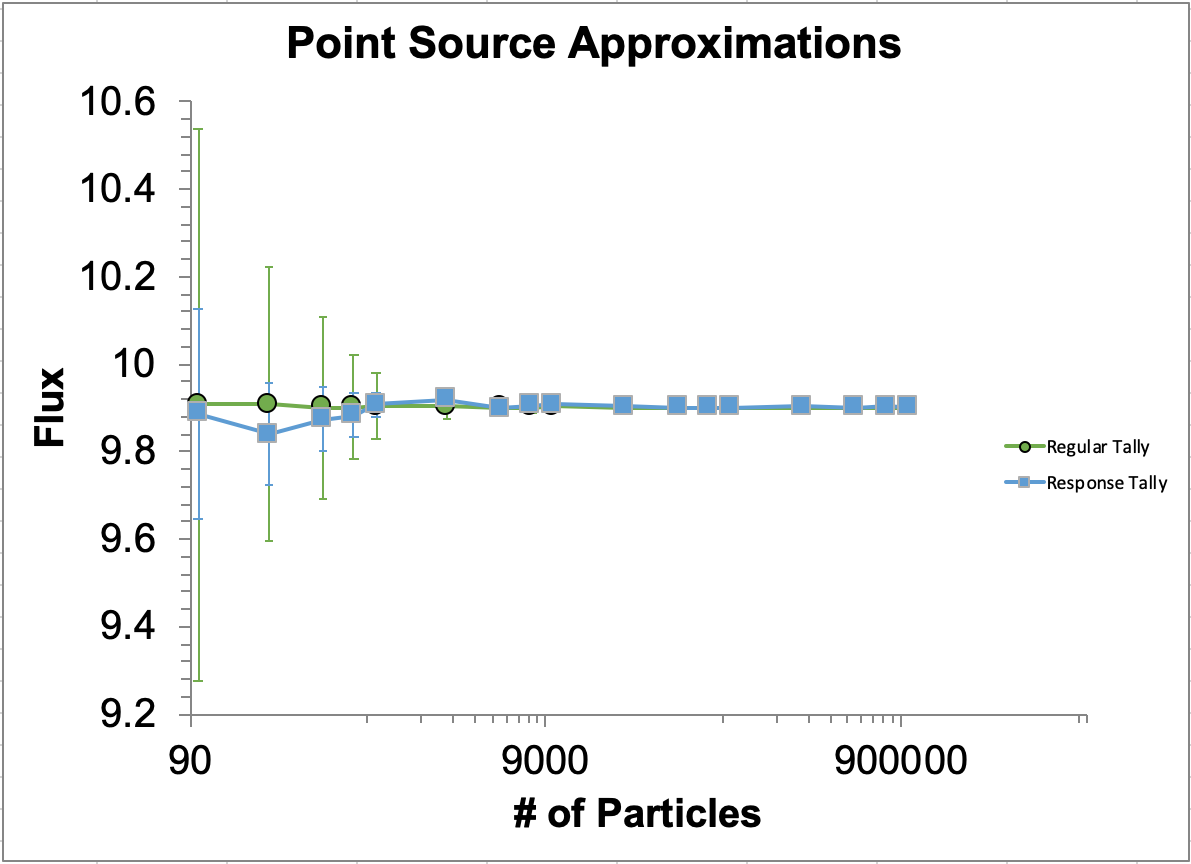
\includegraphics[height=3in]{Figures/point_src_errors.png}
		\caption{A graph showing the average values of the flux for a point source problem as well as the accompanying variance as a function of the number of particles used in the simulation. This shows that our method has far less variance for fewer simulated particles, which implies that it is a more reliable method under these conditions.}
		\label{fig:point_source_errors}
	\end{figure}

	\begin{figure} [h!]
		\centering
		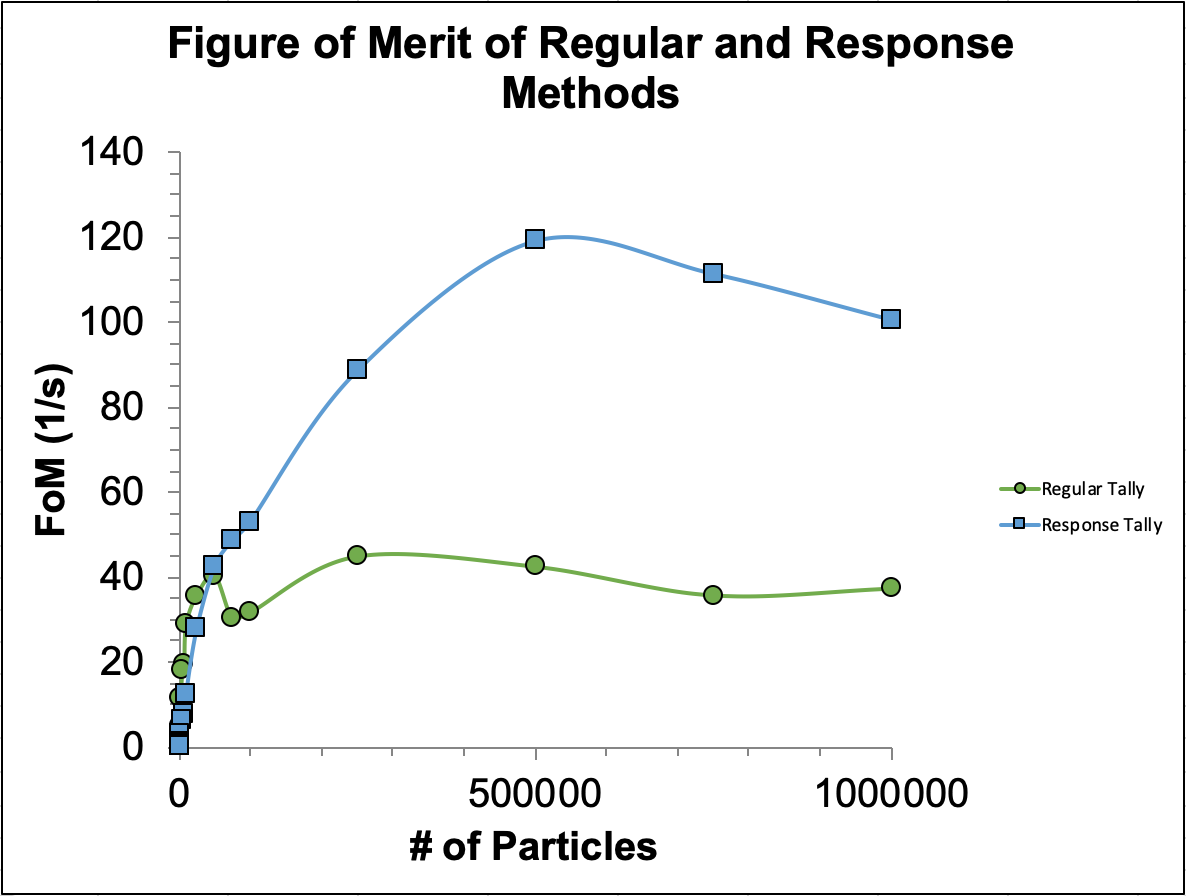
\includegraphics[height=3in]{Figures/point_src_fom.png}
		\caption{A graph showing the figure of merits (FoM) of the regular tally method as well as the response function. A higher FoM corresponds to a method that provides less variance in a more efficient span of time. This figure shows that after approx. 50k particles, our method results in a greatly improved FoM compared to a regular tally. This provides a strong basis for the usefulness of our method.
}
		\label{fig:point_source_FoM}
	\end{figure}

	\begin{figure} [h!]
		\centering
		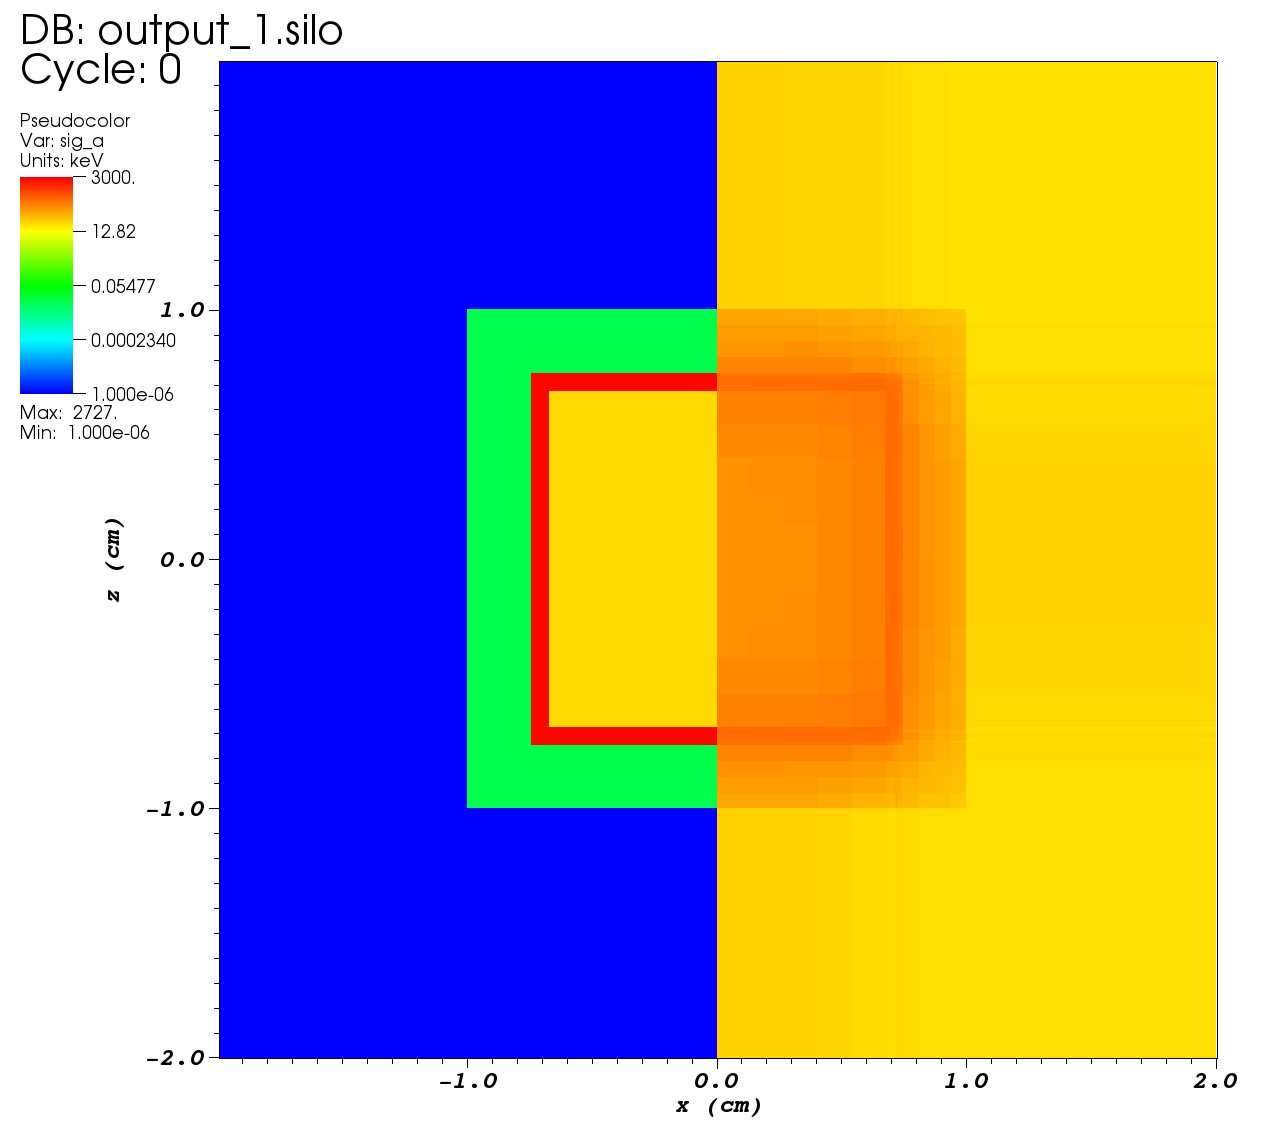
\includegraphics[height=3in]{Figures/cubanova_op_a.png}
		\caption{A plot of the geometrically simplified supernova problem showing the true $\sigma_{a}$ value of the problem (left-hand side) as well as the $\sigma_{r}$ values generated by the response function method (right-hand side). $\sigma_{r}$  represents the average opacity between the cell and every possible tally location. The smearing artifacts show a limitation of the direction-independent $\sigma_{r}$ value calculation; disregarding the  particle directionality while it is traced through the mesh results in some cells receiving a larger $\sigma_{r}$ value.}
		\label{fig:cubanova_op_a}
	\end{figure}

	To check the validity of the response function method, a point source problem was devised where the analytic flux was known.

\section{Results \& Supernova Applications}
	\begin{figure} [h!]
		\centering
		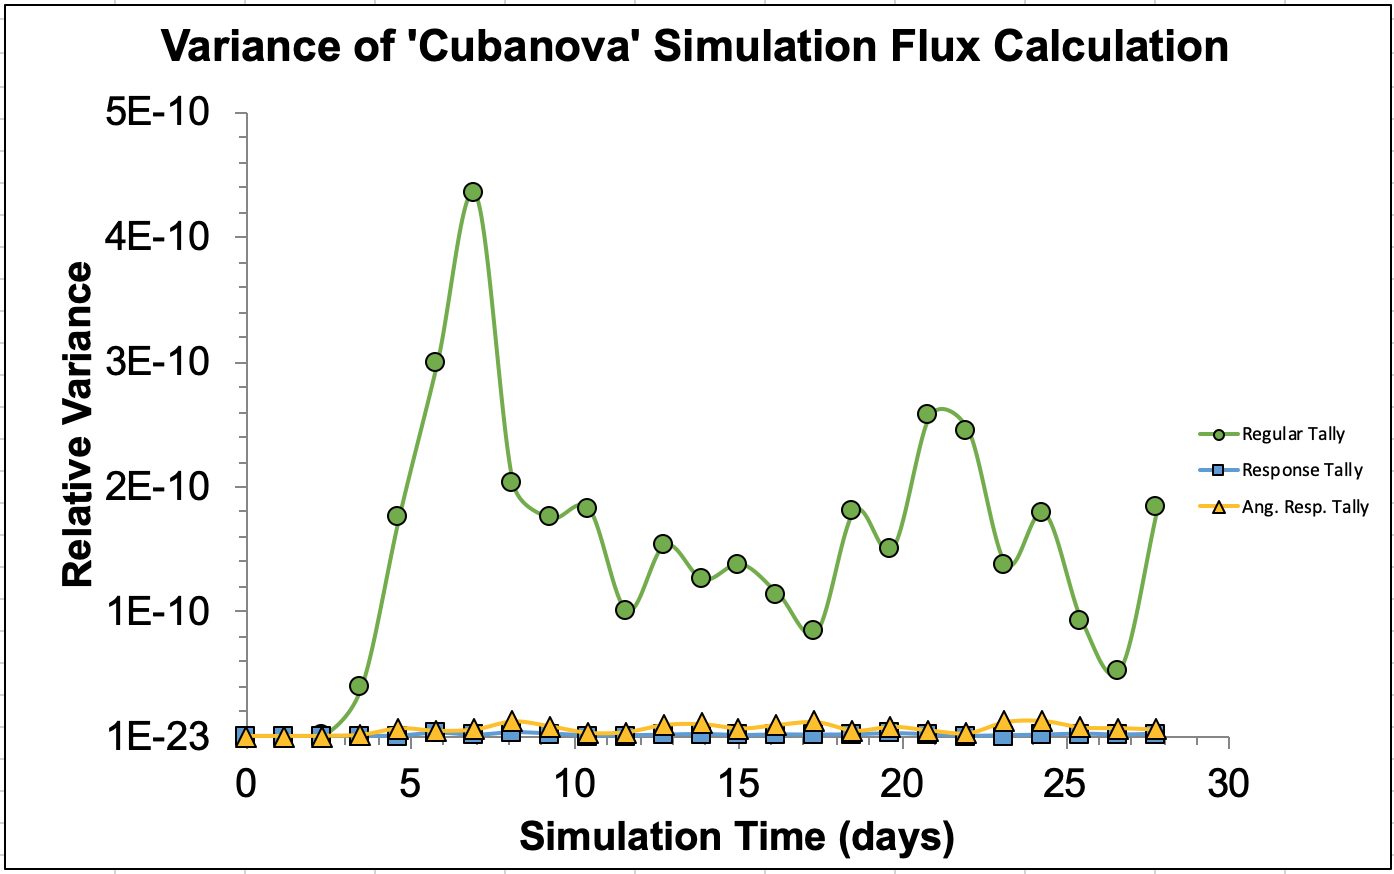
\includegraphics[height=3in]{Figures/cubanova_flux_var.png}
		\caption{A graph demonstrating the variance of the regular tally, and response function tally for the simplified supernova simulation from Fig. \ref{fig:cubanova_op_a} as a function of the simulation time. Twenty independent simulations were run with unique random number seeds. The general trends indicate that the response function method has a significantly lower variance at any given time step compared to the regular tally method.}
		\label{fig:cubanova_flux_var}
	\end{figure}
	
	\begin{figure} [h!]
		\centering
		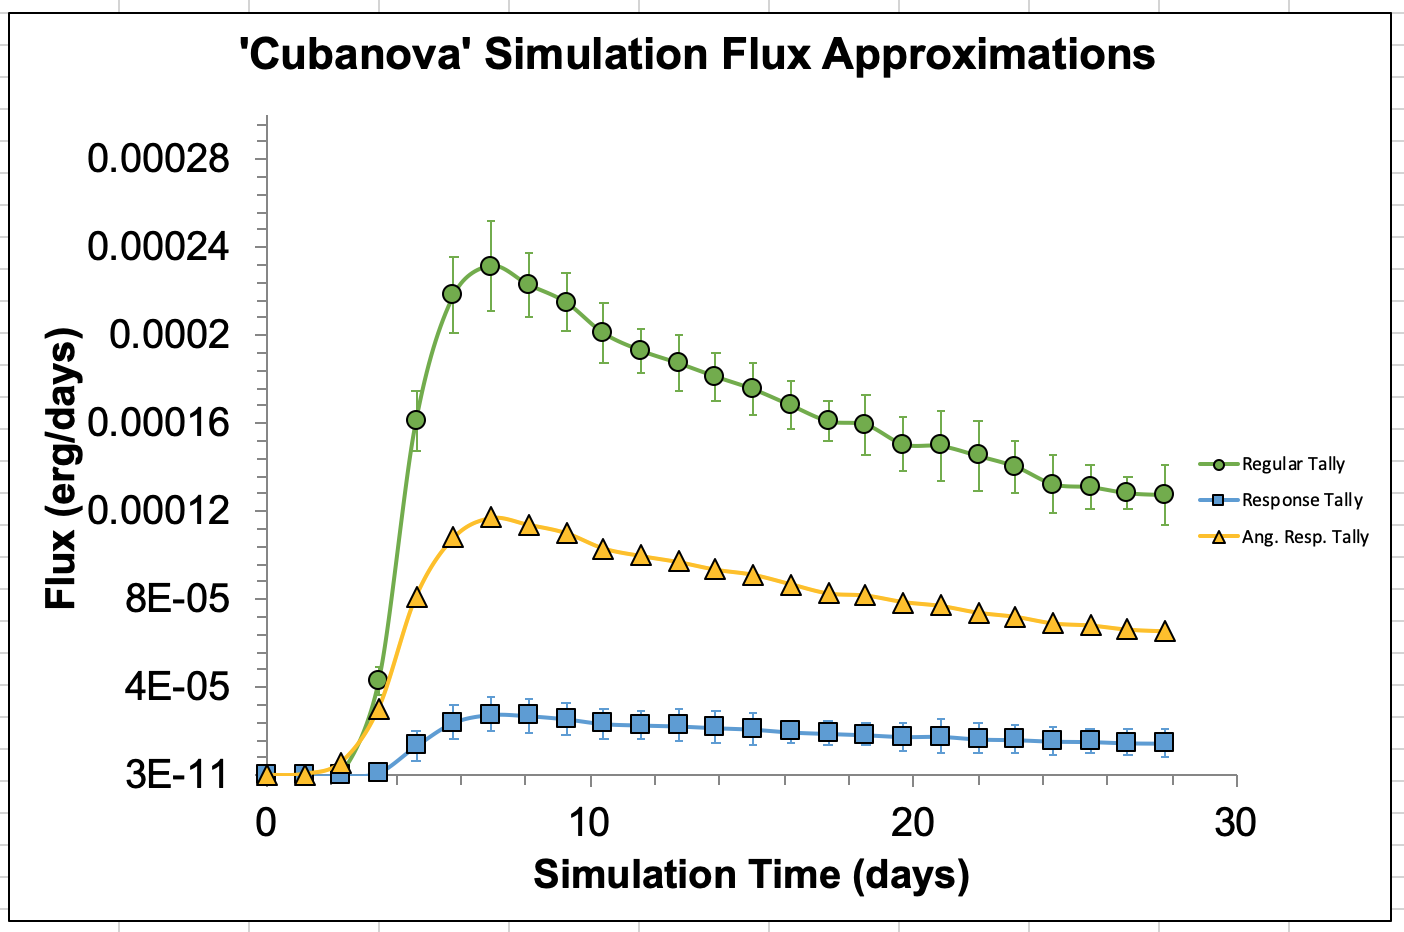
\includegraphics[height=3in]{Figures/cubanova_avg_error.png}
		\caption{The relative flux calculations made by the regular tally method and the response function tally method. As in Fig. \ref{fig:point_source_errors}, the response method has a smaller variance, however, it also drastically underestimates the flux. This likely stems from the use of a spherical tally surface instead of a directional tally surface for this particular problem.}
		\label{fig:cubanova_avg_error}
	\end{figure}
	
	\begin{figure} [h!]
		\centering
		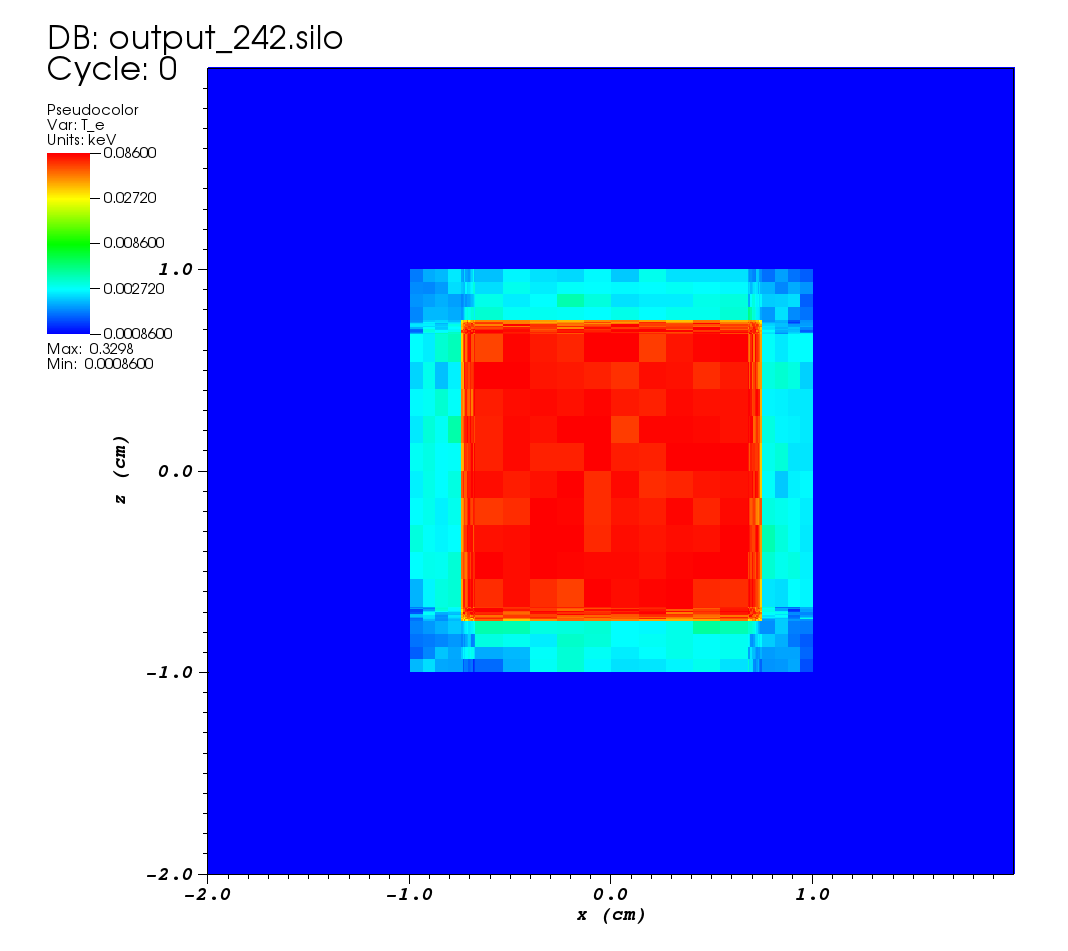
\includegraphics[height=3in]{Figures/cubanova_T_e.png}
		\caption{A plot of the electron temperature at the end of the simulations shown in Figs. \ref{fig:cubanova_op_a}, \ref{fig:cubanova_flux_var}, \ref{fig:cubanova_avg_error}. The overheating likely results from the small corner cells. }
		\label{fig:cubanova_T_e}
	\end{figure}

	\begin{figure} [h!]
		\centering
		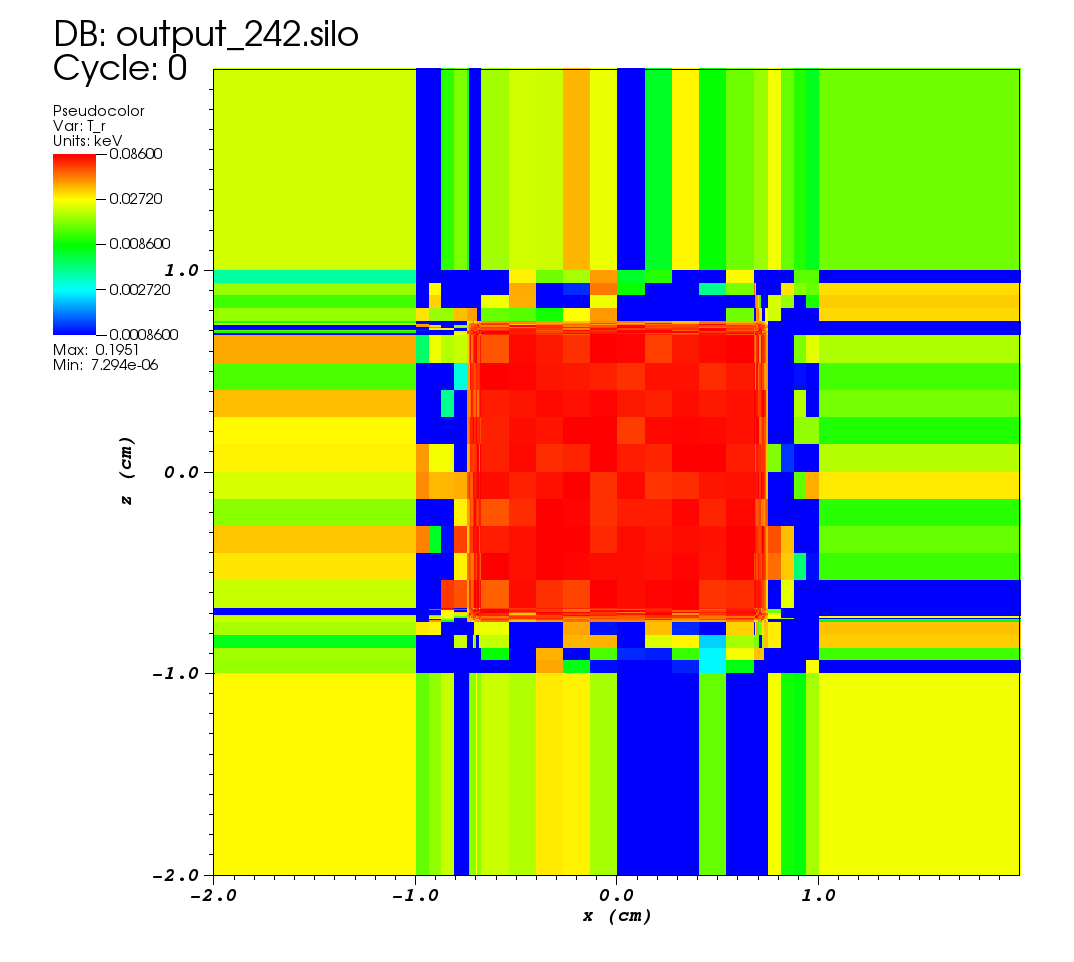
\includegraphics[height=3in]{Figures/cubanova_T_r.png}
		\caption{A plot of the radiation temperature from the plot in Fig. \ref{fig:cubanova_T_e}. The noise in the radiation field results from a limited number of photons, the optical thickness of the material, and the coarse mesh granularity of the void region.}
		\label{fig:cubanova_T_r}
	\end{figure}


\section{Conclusions}


\begin{thebibliography}{99}
\bibitem{FC71} J.A.\ Fleck, Jr.\ and J.D.\ Cummings, Jr., ``An implicit Monte Carlo scheme for calculating time and frequency dependent nonlinear radiation transport,''
  {\em J.\ Comp.\ Phys.} 8, pp.\ 313--342, (1971).
\bibitem{KW09} D.\ Kasen and S.E.\ Woosley, ``Type II supernovae: model light curves and standard candle relationships,''
  {\em ApJ} 703, pp.\ 2205--2216, (2009).
\bibitem{MS10} A.J.\ van Marle, N.\ Smith, S.P\ Owocki, B. van Veelen, ``Numerical models of collisions between core-collapse supernovae and circumstellar shells,''
  {\em MNRAS} 407, pp.\ 2305--2327, (2010).
\bibitem{MK12} A.J.\ van Marle, R.\ Keppens, ``Multi-dimensional models of circumstellar shells around evolved massive stars,''
  {\em A \& A} 547, A3 (2012).
\bibitem{MB13} T.J.\ Moriya, S.I.\ Blinnikov, N.\ Tominaga et al., ``Light-curve modelling of superluminous supernova 2006gy: collision between supernova ejecta and a dense circumstellar medium,''
  {\em MNRAS} 428, pp.\ 1020--1035, (2013).
\bibitem{VL16} A.\ Vlasis, L.\ Dessart, and E.\ Audit, ``Two-dimensional radiation hydrodynamics simulations of superluminous interacting supernovae of Type IIn,''
  {\em MNRAS} 458, pp.\ 1253--1266, (2016).
\bibitem{MP18} A.T.\ McDowell, P.C.\ Duffel, and D.\ Kasen, ``Interaction of a Supernova with a Circumstellar Disk,''
  {\em ApJ} 856, (2018).
\end{thebibliography}

\end{document}
